\PassOptionsToPackage{unicode=true}{hyperref} % options for packages loaded elsewhere
\PassOptionsToPackage{hyphens}{url}
%
\documentclass[]{article}
\usepackage{lmodern}
\usepackage{amssymb,amsmath}
\usepackage{ifxetex,ifluatex}
\usepackage{fixltx2e} % provides \textsubscript
\ifnum 0\ifxetex 1\fi\ifluatex 1\fi=0 % if pdftex
  \usepackage[T1]{fontenc}
  \usepackage[utf8]{inputenc}
  \usepackage{textcomp} % provides euro and other symbols
\else % if luatex or xelatex
  \usepackage{unicode-math}
  \defaultfontfeatures{Ligatures=TeX,Scale=MatchLowercase}
\fi
% use upquote if available, for straight quotes in verbatim environments
\IfFileExists{upquote.sty}{\usepackage{upquote}}{}
% use microtype if available
\IfFileExists{microtype.sty}{%
\usepackage[]{microtype}
\UseMicrotypeSet[protrusion]{basicmath} % disable protrusion for tt fonts
}{}
\IfFileExists{parskip.sty}{%
\usepackage{parskip}
}{% else
\setlength{\parindent}{0pt}
\setlength{\parskip}{6pt plus 2pt minus 1pt}
}
\usepackage{hyperref}
\hypersetup{
            pdftitle={Blue Hunters: Bluetooth RSSI Locator Robots},
            pdfauthor={Jacob Glueck (jng55); Jane Du (zd53); Justin Cray (jgc232)},
            pdfborder={0 0 0},
            breaklinks=true}
\urlstyle{same}  % don't use monospace font for urls
\usepackage{color}
\usepackage{fancyvrb}
\newcommand{\VerbBar}{|}
\newcommand{\VERB}{\Verb[commandchars=\\\{\}]}
\DefineVerbatimEnvironment{Highlighting}{Verbatim}{commandchars=\\\{\}}
% Add ',fontsize=\small' for more characters per line
\newenvironment{Shaded}{}{}
\newcommand{\KeywordTok}[1]{\textcolor[rgb]{0.00,0.44,0.13}{\textbf{#1}}}
\newcommand{\DataTypeTok}[1]{\textcolor[rgb]{0.56,0.13,0.00}{#1}}
\newcommand{\DecValTok}[1]{\textcolor[rgb]{0.25,0.63,0.44}{#1}}
\newcommand{\BaseNTok}[1]{\textcolor[rgb]{0.25,0.63,0.44}{#1}}
\newcommand{\FloatTok}[1]{\textcolor[rgb]{0.25,0.63,0.44}{#1}}
\newcommand{\ConstantTok}[1]{\textcolor[rgb]{0.53,0.00,0.00}{#1}}
\newcommand{\CharTok}[1]{\textcolor[rgb]{0.25,0.44,0.63}{#1}}
\newcommand{\SpecialCharTok}[1]{\textcolor[rgb]{0.25,0.44,0.63}{#1}}
\newcommand{\StringTok}[1]{\textcolor[rgb]{0.25,0.44,0.63}{#1}}
\newcommand{\VerbatimStringTok}[1]{\textcolor[rgb]{0.25,0.44,0.63}{#1}}
\newcommand{\SpecialStringTok}[1]{\textcolor[rgb]{0.73,0.40,0.53}{#1}}
\newcommand{\ImportTok}[1]{#1}
\newcommand{\CommentTok}[1]{\textcolor[rgb]{0.38,0.63,0.69}{\textit{#1}}}
\newcommand{\DocumentationTok}[1]{\textcolor[rgb]{0.73,0.13,0.13}{\textit{#1}}}
\newcommand{\AnnotationTok}[1]{\textcolor[rgb]{0.38,0.63,0.69}{\textbf{\textit{#1}}}}
\newcommand{\CommentVarTok}[1]{\textcolor[rgb]{0.38,0.63,0.69}{\textbf{\textit{#1}}}}
\newcommand{\OtherTok}[1]{\textcolor[rgb]{0.00,0.44,0.13}{#1}}
\newcommand{\FunctionTok}[1]{\textcolor[rgb]{0.02,0.16,0.49}{#1}}
\newcommand{\VariableTok}[1]{\textcolor[rgb]{0.10,0.09,0.49}{#1}}
\newcommand{\ControlFlowTok}[1]{\textcolor[rgb]{0.00,0.44,0.13}{\textbf{#1}}}
\newcommand{\OperatorTok}[1]{\textcolor[rgb]{0.40,0.40,0.40}{#1}}
\newcommand{\BuiltInTok}[1]{#1}
\newcommand{\ExtensionTok}[1]{#1}
\newcommand{\PreprocessorTok}[1]{\textcolor[rgb]{0.74,0.48,0.00}{#1}}
\newcommand{\AttributeTok}[1]{\textcolor[rgb]{0.49,0.56,0.16}{#1}}
\newcommand{\RegionMarkerTok}[1]{#1}
\newcommand{\InformationTok}[1]{\textcolor[rgb]{0.38,0.63,0.69}{\textbf{\textit{#1}}}}
\newcommand{\WarningTok}[1]{\textcolor[rgb]{0.38,0.63,0.69}{\textbf{\textit{#1}}}}
\newcommand{\AlertTok}[1]{\textcolor[rgb]{1.00,0.00,0.00}{\textbf{#1}}}
\newcommand{\ErrorTok}[1]{\textcolor[rgb]{1.00,0.00,0.00}{\textbf{#1}}}
\newcommand{\NormalTok}[1]{#1}
\usepackage{longtable,booktabs}
% Fix footnotes in tables (requires footnote package)
\IfFileExists{footnote.sty}{\usepackage{footnote}\makesavenoteenv{longtable}}{}
\usepackage{graphicx,grffile}
\graphicspath{{../assets/}{../renderings/}}
\makeatletter
\def\maxwidth{\ifdim\Gin@nat@width>\linewidth\linewidth\else\Gin@nat@width\fi}
\def\maxheight{\ifdim\Gin@nat@height>\textheight\textheight\else\Gin@nat@height\fi}
\makeatother
% Scale images if necessary, so that they will not overflow the page
% margins by default, and it is still possible to overwrite the defaults
% using explicit options in \includegraphics[width, height, ...]{}
\setkeys{Gin}{width=\maxwidth,height=\maxheight,keepaspectratio}
\setlength{\emergencystretch}{3em}  % prevent overfull lines
\providecommand{\tightlist}{%
  \setlength{\itemsep}{0pt}\setlength{\parskip}{0pt}}
\setcounter{secnumdepth}{0}
% Redefines (sub)paragraphs to behave more like sections
\ifx\paragraph\undefined\else
\let\oldparagraph\paragraph
\renewcommand{\paragraph}[1]{\oldparagraph{#1}\mbox{}}
\fi
\ifx\subparagraph\undefined\else
\let\oldsubparagraph\subparagraph
\renewcommand{\subparagraph}[1]{\oldsubparagraph{#1}\mbox{}}
\fi

% set default figure placement to htbp
\makeatletter
\def\fps@figure{htbp}
\makeatother


\title{Blue Hunters: Bluetooth RSSI Locator Robots}
\providecommand{\subtitle}[1]{}
\subtitle{\emph{ECE 4760, Fall 2017}}
\author{Jacob Glueck (\href{mailto:jng55@cornell.edu}{jng55}) \and Jane Du (\href{mailto:zd53@cornell.edu}{zd53}) \and Justin Cray (\href{mailto:jgc232@cornell.edu}{jgc232})}
\date{December 6, 2017}

\begin{document}
\maketitle

\hypertarget{introduction}{%
\subsection{Introduction}\label{introduction}}

Position estimation and navigation for robots is an interesting problem
in the field of robotics. We investigate the challenge of determining
relative position using signal strength; by placing a moving robot on
the same plane as a beacon, oriented and positioned randomly, the
robot can hunt out and move towards the beacon by itself. We discuss 
our procedures and challenges we encountered in this article.

Specifically, we built 2 small cars which used Bluetooth Received Signal Strength
Indicator (RSSI) measurements to navigate towards a stationary base
station. The cars and base station used a Bluetooth Low Energy (BLE) 4.0
module to take the measurements and a PIC32MX250 microcontroller. The
cars also used a 3 axis magnetometer as as compass in order to reliably
turn, as well as 2 micro 9 g servos to drive. Each unit was powered with
3 AA batteries. Finally, the chassis and wheels of each car were 3D
printed.

\hypertarget{design}{%
\subsection{Design}\label{design}}

The design of the project can be split into 3 main parts: the chassis, the electronics (hardware), and the software. The following sections discuss implementation details.

\hypertarget{chassis}{%
\subsubsection{Chassis}\label{chassis}}

The robots are made from 4 3D printed pieces: 2 wheels, the frame, and
the caster in the back. The servos, a 3 AA battery holder, and a
perfboard containing all the circuitry are mounted directly to the
frame.

The robots where designed in \href{http://www.openscad.org/}{OpenSCAD},
and their source code is available in
\href{https://github.com/orangeturtle739/bluehunters/tree/master/cad}{our
git repository} and
\protect\hyperlink{appendix-b-source-listing}{below}. There are three
files, \href{generated/frame.scad.html}{\texttt{frame.scad}},
\href{generated/drag.scad.html}{\texttt{drag.scad}}, and
\href{generated/wheel.scad.html}{\texttt{wheel.scad}}, for each of the
three parts. The main modules are defined in
\href{generated/main.scad.html}{\texttt{main.scad}}, and the other files
just instantiate them. The following renderings show each part:

\begin{figure}
\centering
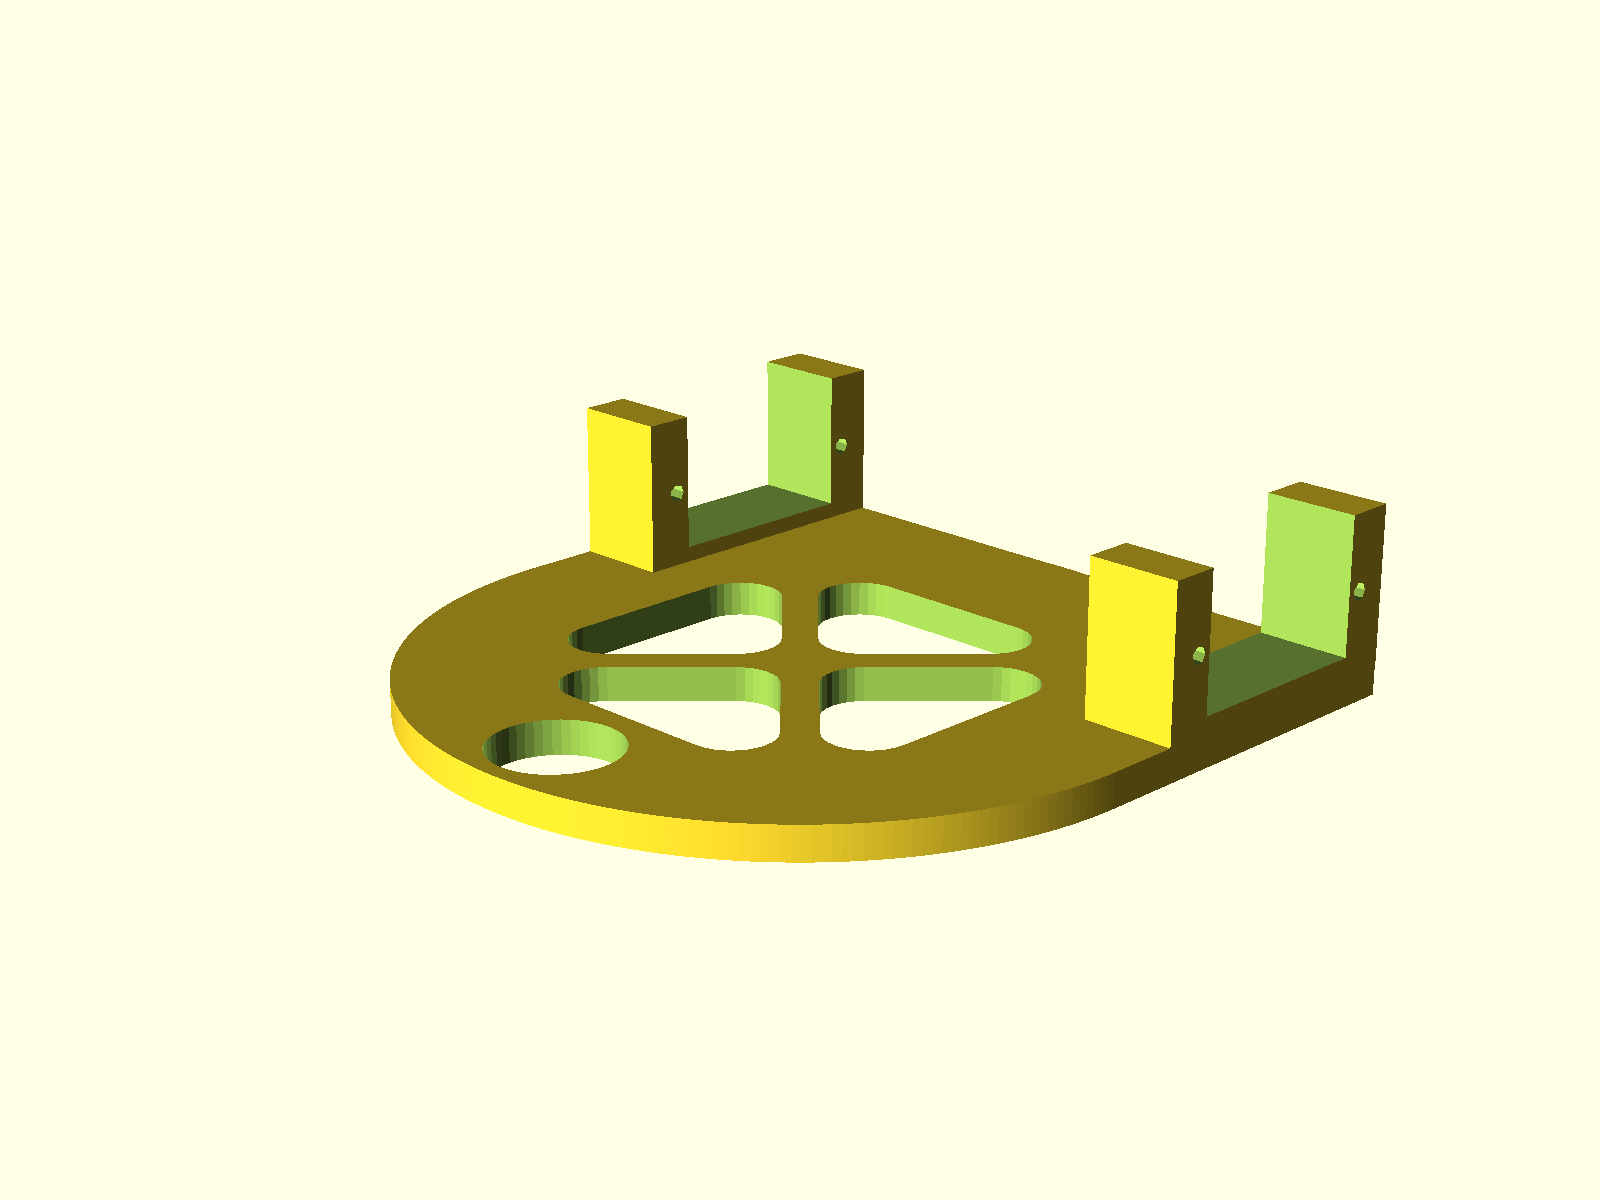
\includegraphics[width=0.5\textwidth,height=\textheight]{frame.png}
\caption{Robot chassis}
\end{figure}

\begin{figure}
\centering
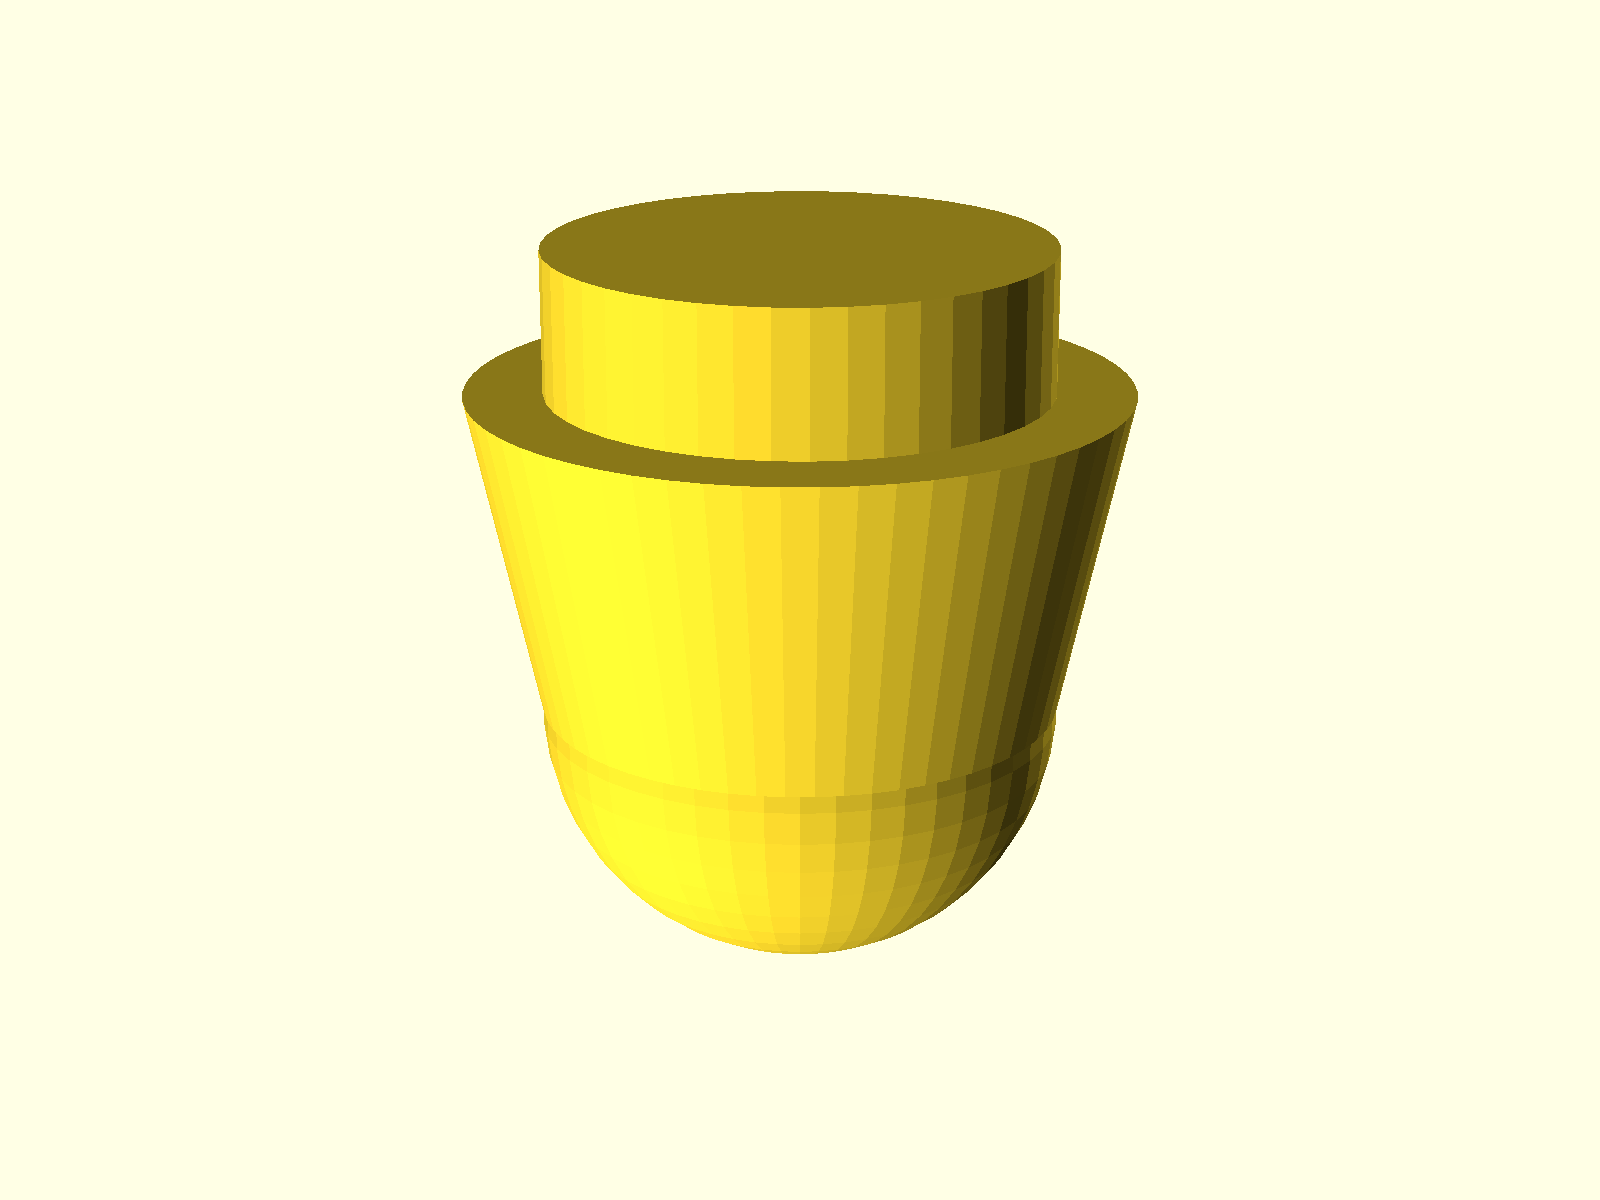
\includegraphics[width=0.5\textwidth,height=\textheight]{drag.png}
\caption{Caster wheel on back of robot}
\end{figure}

\begin{figure}
\centering
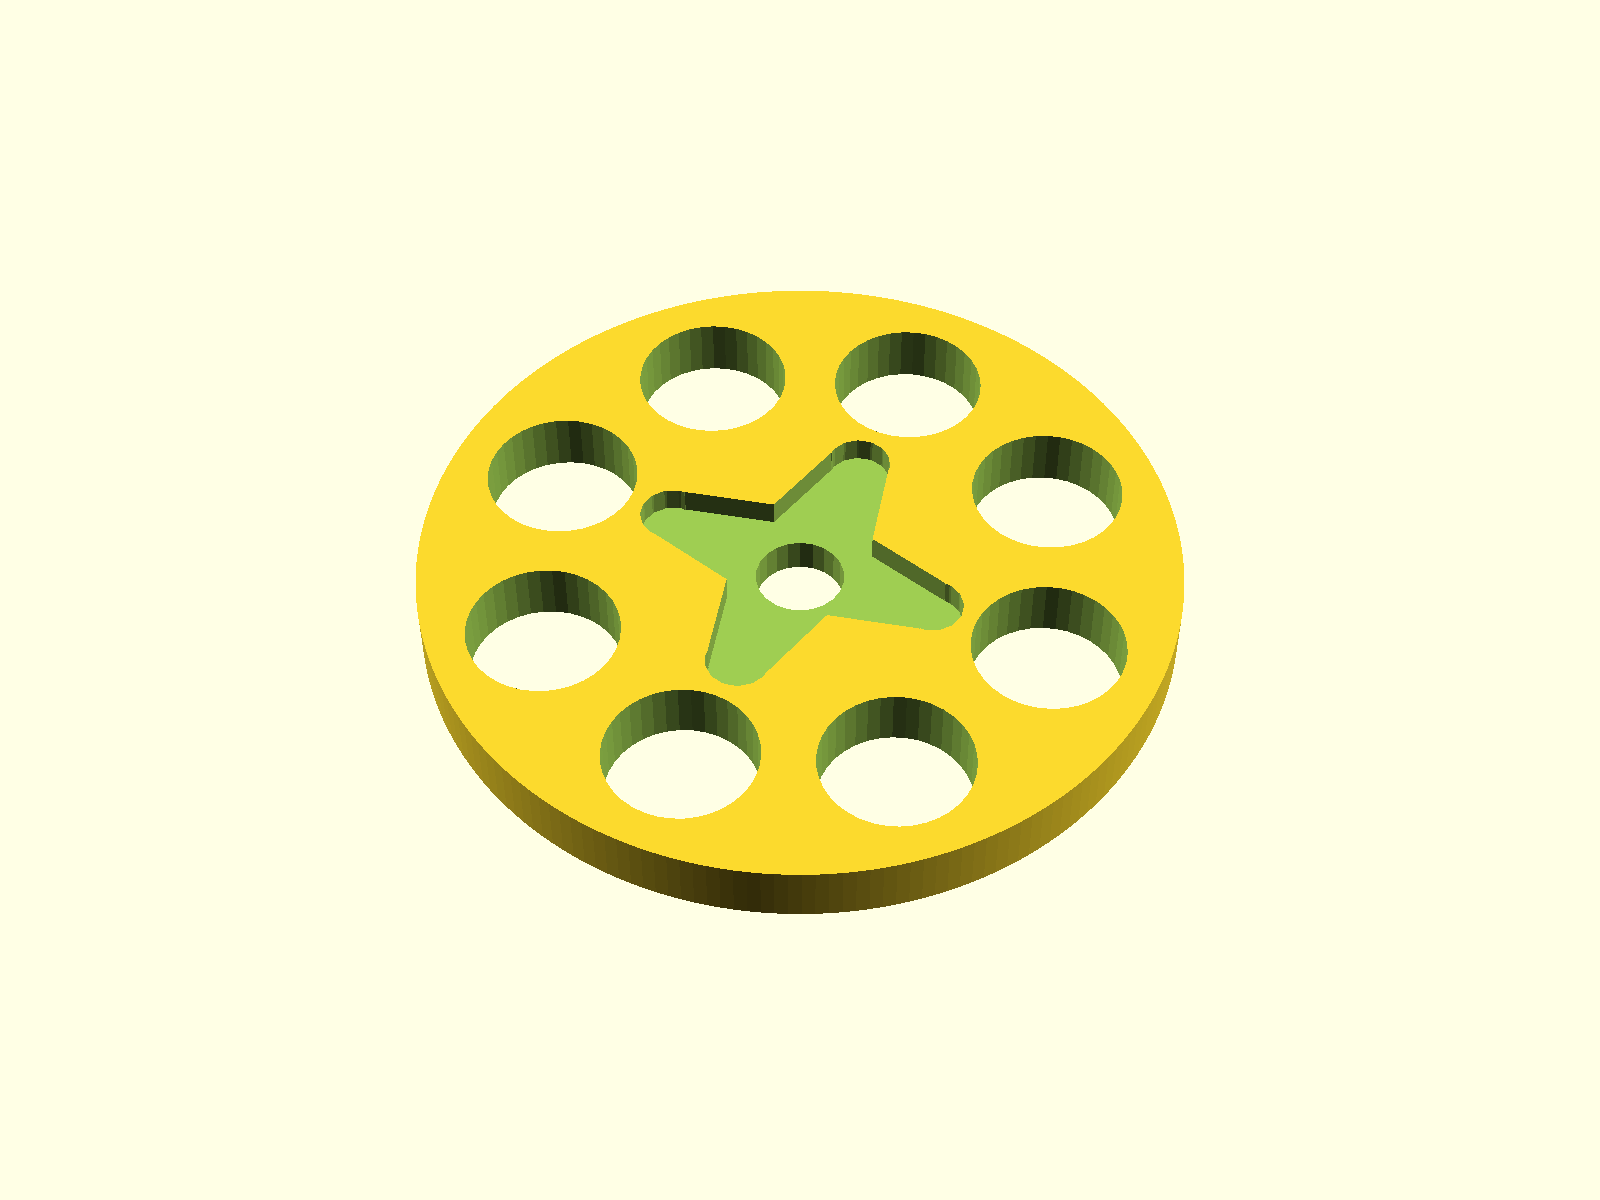
\includegraphics[width=0.5\textwidth,height=\textheight]{wheel.png}
\caption{Robot wheel}
\end{figure}

The parts were printed in ABS using
\href{https://www.monoprice.com/product?c_id=107\&cp_id=10724\&cs_id=1072403\&p_id=13860\&seq=1\&format=2}{Maker
Select 3D Printer v2} printers. All parts were printed with a layer
height of 0.3 mm, as there was no need for a smooth finish or high
tolerances. The parts where sliced with
\href{https://ultimaker.com/en/products/ultimaker-cura-software}{Cura}.

\hypertarget{pictures}{%
\subsubsection{Pictures}\label{pictures}}

Full system (base station and 2 robots):

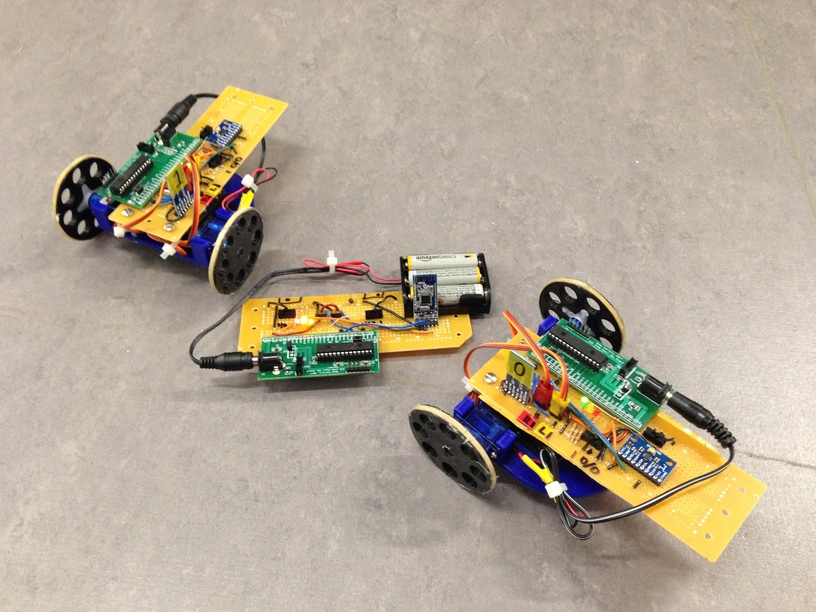
\includegraphics[width=0.5\textwidth,height=\textheight]{full_system.jpg}

Multiple views of the robots:

\begin{longtable}[]{@{}ll@{}}
\toprule
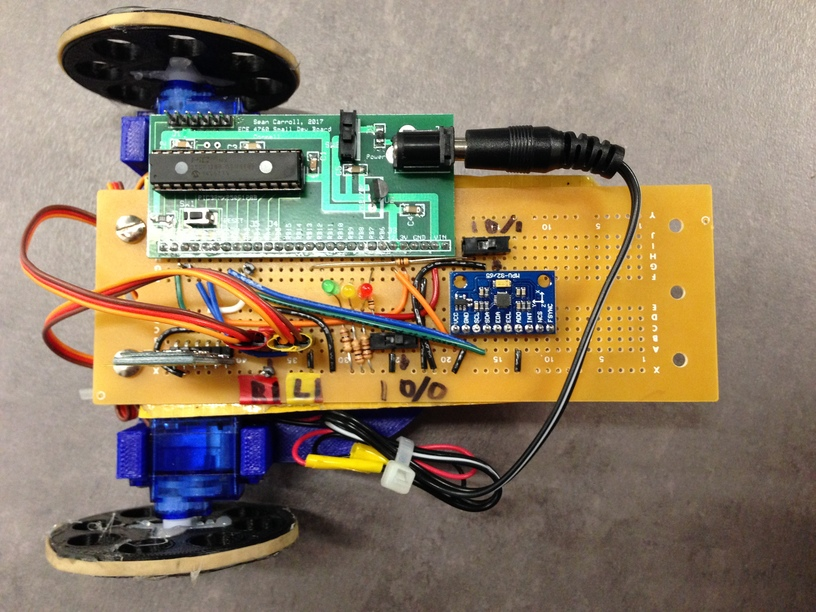
\includegraphics{top_view.jpg} &
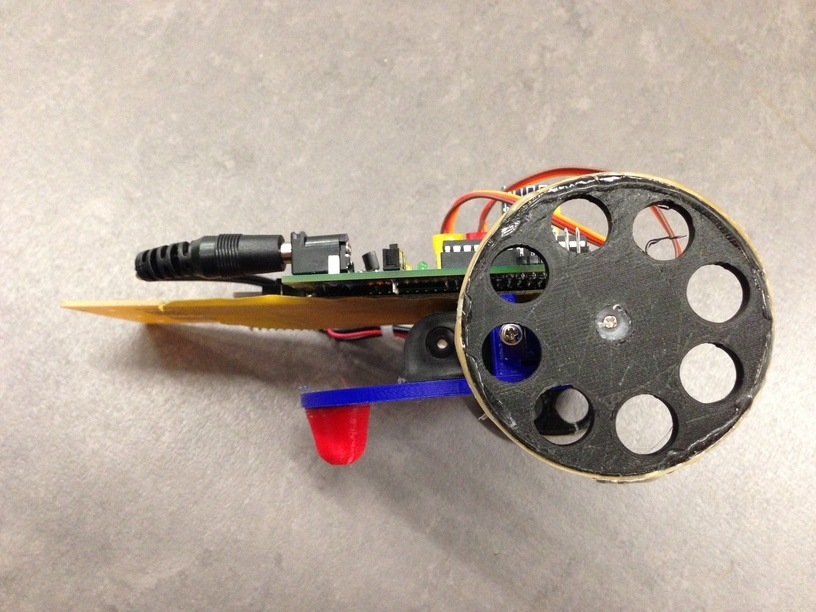
\includegraphics{side_view.jpg}\tabularnewline
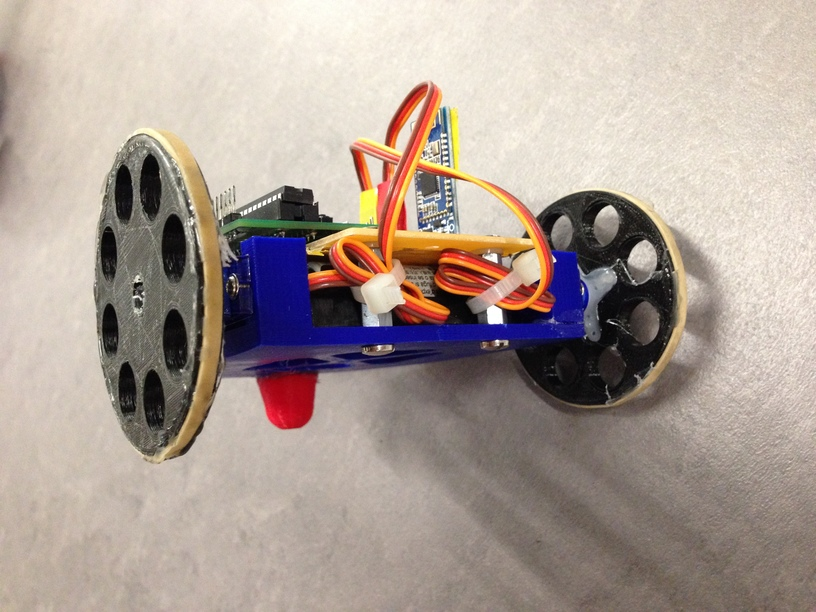
\includegraphics{front_view.jpg} &
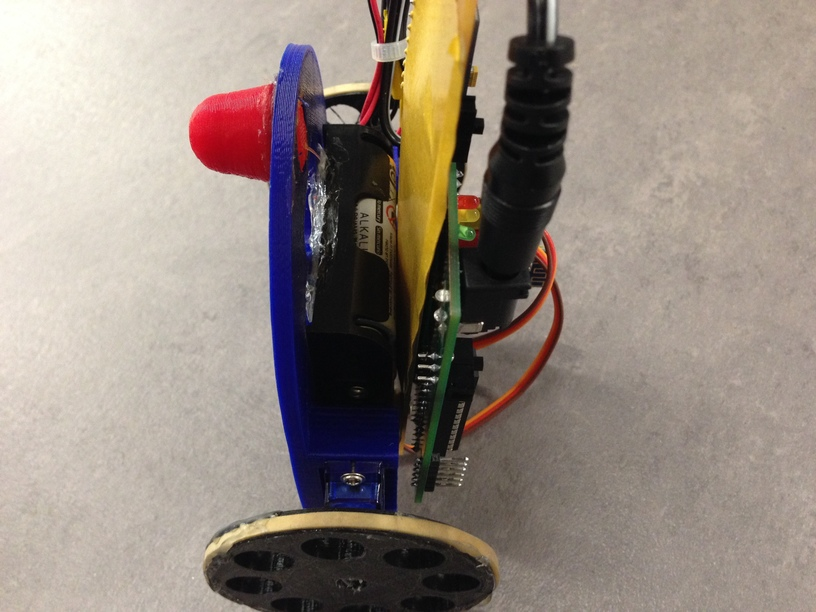
\includegraphics{inside_view.jpg}\tabularnewline
\bottomrule
\end{longtable}

\hypertarget{electronics}{%
\subsubsection{Electronics}\label{electronics}}

\hypertarget{bluetooth-modules}{%
\paragraph{Bluetooth modules}\label{bluetooth-modules}}

The HM-10 bluetooth modules we bought off Ebay were fakes: they were not
made by Jnhuamao \footnote{Jnhuamao is the company which makes the HM-10
  module, along with other Bluetooth modules. Their English website is:
  \url{http://www.jnhuamao.cn/bluetooth.asp?id=1}.}, and did not come
with genuine Jnhuamao firmware. However, they did have real TI CC2541
chips. We realized they were fakes when they did not behave according to
the Jnhuamao data sheet (see \protect\hyperlink{data-sheets}{the data
sheets section}). Luckily, the hardware on the fake chips is the same as
that of the genuine chips, minus an external crystal, and the genuine
firmware checks for the presence of the crystal, and works even without
it. \footnote{\url{http://forum.arduino.cc/index.php?topic=393655.msg2709528\#msg2709528}.}
As such, we reprogrammed the chips with the genuine firmware according
to an
\href{http://forum.arduino.cc/index.php?topic=393655.msg2709528\#msg2709528}{Arduino
forum post}:

\begin{enumerate}
\def\labelenumi{\arabic{enumi}.}
\item
  We soldered wires to the programming pins on the breakout boards, and
  connected those pins to an
  \href{https://www.pjrc.com/teensy/teensy31.html}{Arduino Teensy 3.2}.
  We chose a Teensy because it is 3.3 V as opposed to 5, which would
  damage the 3.3 V CC2541.

  The pins were connected as follows:

  \begin{longtable}[]{@{}lll@{}}
  \toprule
  Name & CC2541 Pin & Arduino Pin\tabularnewline
  \midrule
  \endhead
  \texttt{DEBUG\_CLOCK} & 7 & 5\tabularnewline
  \texttt{DEBUG\_DATA} & 8 & 6\tabularnewline
  \texttt{RESET\_N} & 11 & 4\tabularnewline
  \bottomrule
  \end{longtable}

  The layout of the HM-10 board is:

  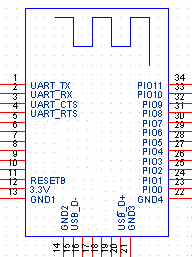
\includegraphics{hm10_pins.png}
\item
  We uploaded the
  \href{https://github.com/RedBearLab/CCLoader/blob/master/Arduino/CCLoader/CCLoader.ino}{\texttt{CCLoader.ino}
  sketch} to the Arduino.
\item
  Finally, we ran (in a Windows virtual machine)
  \href{https://github.com/RedBearLab/CCLoader/tree/master/Windows}{\texttt{CCLoader.exe}}.
  This program takes 3 arguments:

\begin{Shaded}
\begin{Highlighting}[]
\ExtensionTok{CCLoader.exe} \OperatorTok{<}\NormalTok{COM Port}\OperatorTok{>} \OperatorTok{<}\NormalTok{Firmware.bin}\OperatorTok{>}\NormalTok{ 0}
\end{Highlighting}
\end{Shaded}

  The firmware file came from the same Arduino form post, and can be
  found
  \href{http://forum.arduino.cc/index.php?action=dlattach;topic=393655.0;attach=183702}{here}.
\end{enumerate}

There is also an excellent
\href{https://www.youtube.com/watch?v=ez3491-v8Og}{YouTube video}, which
explains the firmware flashing process.

After flashing genuine firmware onto the chip, the next step was to
update the firmware to the latest version. The firmware flashed onto the
board was version 540, but Jnhuamao had (at the time we did this
project)
\href{http://www.jnhuamao.cn/rom/HMSoft-10-2541-V603.zip}{released
version 603}. \footnote{Jnhuamao's firmware download page
  \url{http://www.jnhuamao.cn/download_rom_en.asp?id=1\#}.} They also
provide
\href{http://www.jnhuamao.cn/HowToUpgradeFirmware_en.zip}{instructions
on how to upgrade the firmware}. The basic process is:

\begin{enumerate}
\def\labelenumi{\arabic{enumi}.}
\tightlist
\item
  Connect the HM-10 module to a computer using a 3.3 V FTDI to USB
  adapter. Then, use PUTTY to establish a serial session (9600 baud,
  8N1). Send the chip \texttt{AT}; if it is connected properly, it will
  respond with \texttt{OK}.
\item
  Send the chip \texttt{AT+SBLUP} to put it in firmware update mode. It
  will respond with \texttt{OK+SBLUP}. Terminate the PUTTY session.
\item
  Run the \texttt{HMSoft.exe} program distributed in the firmware update
  download. We ran it in a Windows virtual machine because we did not
  trust it.
\item
  Select the proper port and firmware file using the software, and hit
  ``Load Image''. The software should handle the rest!
\item
  To make sure it worked, establish a serial connection again using
  PUTTY. Send \texttt{AT+VERS?} to query the chip for version
  information.
\end{enumerate}

\hypertarget{software}{%
\subsubsection{Software}\label{software}}

The robots were programmed in C, using the
\href{http://www.microchip.com/mplab/mplab-x-ide}{MPLAB X IDE} v4.0,
with the \href{http://www.microchip.com/mplab/compilers}{XC32} v1.4
compiler and the
\href{http://www.microchip.com/SWLibraryWeb/product.aspx?product=PIC32\%20Peripheral\%20Library}{PIC
32 Legacy Peripheral Library (plib)}. The full source code is available
in
\href{https://github.com/orangeturtle739/bluehunters/tree/master/ble.X}{our
git repository} and
\protect\hyperlink{appendix-b-source-listing}{below}. The code is
divided into 5 main units:

\begin{itemize}
\tightlist
\item
  \href{generated/ble.c.html}{\texttt{ble.c}}: contains all the
  functions for interacting with the BLE device over UART.
\item
  \href{generated/imu.c.html}{\texttt{imu.c}}: contains all the
  functions for interacting with the IMU (which contained the
  magnetometer) over I2C.
\item
  \href{generated/servo.c.html}{\texttt{servo.c}}: contains all the
  functions for interacting with the servos using PWM.
\item
  \href{generated/main.c.html}{\texttt{main.c}}: the main code.
\item
  \href{generated/pt_cornell_1_2_2.c.html}{\texttt{pt\_cornell\_1\_2\_2.c}}:
  contains the functions which were originally declared in the
  protothreads header file. However, since they were in the header file,
  if multiple source files included the header file, there would be
  linking errors due to duplicate definitions of symbols. Moving the
  protothreads definitions to a separate file resolved this issue.
\end{itemize}

\hypertarget{ble}{%
\paragraph{BLE}\label{ble}}

The BLE module used UART, at 9600 baud 8N1. We used \texttt{UART1} on
the PIC for communicating with the BLE module, and used \texttt{UART2}
for communicating with the computer (for debugging). The BLE files
define a series of macros and \texttt{PT\_THREAD} functions for printing
characters and reading lines in a non-blocking fashion using
protothreads. All of the \texttt{PT\_THREAD} functions can be spawned
with \texttt{PT\_SPAWN} to run them.

The \href{generated/main.c.html}{\texttt{main.c}} file contains a thread
which does all the communication with the Bluetooth chip using these
functions. The commands it sends to the chip are:

\begin{itemize}
\item
  \texttt{AT+RESET}: resets the chip to ensure it is in a clean state
  before receiving other commands.
\item
  \texttt{AT+IBEA1}: enables the iBeacon functionality of the chip (sets
  it to 1; \texttt{AT+IBEA0} would disable it by setting it to 0). This
  allows the chip to be found with an RSSI scan. After setting the
  value, we query it with \texttt{AT+IBEA?} and send the result over the
  other serial port to a computer for debugging.
\item
  \texttt{AT+ROLE0} or \texttt{AT+ROLE1}: sets the role to either
  peripheral (0) or central (1). The base station is set to peripheral,
  and the 2 robots are set to central. Peripheral means the device will
  respond in inquiries from a central device. This allows it to be
  discovered during an RSSI scan. After setting the value, we query it
  with \texttt{AT+ROLE?} and send the result over the other serial port
  to a computer for debugging.
\item
  \texttt{AT+IMME0} or \texttt{AT+IMME1}: sets the work state of the
  device to either actively listening for Bluetooth signals (0), or only
  acting when it receives a serial command (1). Once again, the base
  station is set to 0: it needs to listen for signals and respond. The
  robots are set to 1, as the chips need to initiate scan requests when
  they receive the command over serial. After setting the value, we
  query it with \texttt{AT+IMME?} and send the result over the other
  serial port to a computer for debugging.
\item
  \texttt{AT+NAME\%s}: sets the name of the chip (which is visible when
  scanning) to \texttt{\%s} (For example, \texttt{AT+NAMEPIRATE} names
  the chip \texttt{PIRATE}). We give all the chips unique names to make
  debugging easier. After setting the value, we query it with
  \texttt{AT+NAME?} and send the result over the other serial port to a
  computer for debugging.
\item
  \texttt{AT+SHOW3}: configures the device to advertise both its name
  and RSSI when scanning.
\item
  \texttt{AT+ADDR?}: queries the device for its hardware address. We
  recorded the hardware device of each chip, as when doing RSSI scans,
  the results are reported by hardware address.
\item
  \texttt{AT+DISI?}: performed only on the robots, causing a discovery
  scan. The result of the scan is a bunch of lines of the form:

\begin{verbatim}
OK+DISC:00000000:00000000000000000000000000000000:0000000000:6832A3801EBE:-080
\end{verbatim}

  The second to last token, \texttt{6832A3801EBE}, is the hardware
  address of the discovered device, and the last token, \texttt{-080},
  is the measured RSSI. The chip will transmit a line for each device it
  finds (``line'' is a misnomer as it does not separate them with any
  characters), followed by \texttt{OK+DISCE}.
\end{itemize}

One interesting thing to note about the chip is that commands do not
have to end with newlines or carriage returns. However, if sent, the
chip will ignore them.

\hypertarget{imu}{%
\paragraph{IMU}\label{imu}}

The PIC commmunicates with the IMU via I2C. The IMU includes a breakout
board for the QFN MPU-9250 module, which itself includes 2 dies. One
contains the 3-axis gyroscope and 3-axis accelerometer, which were not
used in this project, and the other die is the AK8963 3-axis
magnetometer (compass).

It is connected to the rest of the MPU module via an auxillary I2C bus,
so it is not connected to the MPU's main I2C bus by default. While the
accelerometer and gyroscope registers can be read after powering up the
IMU, the compass also needs pass-through mode to be enabled on the IMU
to make it an accessible slave on the I2C bus.

Some useful functions as defined in
\href{generated/imu.h.html}{\texttt{imu.h}} are described below:

\begin{itemize}
\tightlist
\item
  \texttt{void\ imu\_init()}: Initializes the MPU-9250, including
  configuring the chip to allow reading the compass.
\item
  \texttt{int\ imu\_get\_heading()} Returns the heading of the robot as
  a value between -180 and 180. The compasses were not completely
  calibrated to find magnetic north; it only ensures angles are correct
  relevant to past headings.
\item
  \texttt{void\ imu\_mag\_read\_data(int\ *\ destination)} Fetches
  compass readings; saves register values into \texttt{destination} in
  the form \texttt{{[}x,\ y,\ z{]}}.
\item
  \texttt{int\ angle\_diff(int\ source,\ int\ target)} Gets the
  difference between two angles in degrees to account for discontinuity
  between -180 and 180 degrees.
\item
  \texttt{int\ degree(int\ deg)}: Offsets degree values so that they
  fall within the range -180 to 180 degrees.
\end{itemize}

Initializing the IMU involves opening the I2C module, and then
configuring the IMU.

\begin{enumerate}
\def\labelenumi{\arabic{enumi}.}
\tightlist
\item
  We open the \texttt{I2C2} module; \texttt{I2C1} uses pins already used
  by the connections to the Bluetooth module. We open it with the baud
  rate generator value
  \texttt{BRG\ =\ (Fpb\ /\ 2\ /\ baudrate)\ -\ 2\ =\ 4e7\ /\ 2\ /\ 4e5\ -\ 2\ =\ 48},
  as specified for \texttt{OpenI2C2()} in the
  \protect\hyperlink{references}{peripheral libraries}.
\item
  Pass through is enabled, interrupts for data ready are enabled, the
  IMU as an I2C master function is disabled, and the sensor is powered
  up.
\end{enumerate}

This enables the PIC to talk to the AK8963. The AK8963 has several modes
of operation, and the chip must be set to power-down mode before
switching to other modes. We read compass values with single measurement
mode, as specified below:

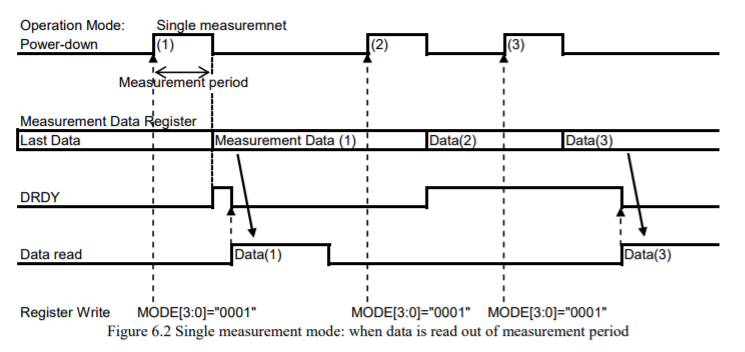
\includegraphics{imu_single_measurement.png}

\begin{enumerate}
\def\labelenumi{\arabic{enumi}.}
\tightlist
\item
  Set the compass to single measurement mode in 14 bit resolution.
\item
  Read the 6 data registers (X low, X high, Y low, Y high, Z low, Z
  high)
\item
  Read the Status 2 register to check for magnetic sensor overflow.
  Without reading this register, the read is not considered complete and
  further reads will fail.
\item
  Wait; if the IMU is read too frequently, it will not have enough time
  to take measurements.
\end{enumerate}

Additional helper methods used in I2C were defined in
\href{generated/imu.c.html}{\texttt{imu.c}}. These are largely based on
the files from the
\protect\hyperlink{code-and-designs-borrowed-from-others}{self-balancing
robot}.

\begin{itemize}
\tightlist
\item
  \texttt{char\ i2c\_read\_device(char\ device,\ char\ address)} Reads
  the data from a single register at \texttt{address}
\item
  \texttt{void\ i2c\_write\_byte(char\ device,\ char\ address,\ char\ data)}
  All configurations used in this project involved writing single bytes
  of data.
\item
  \texttt{void\ i2c\_wait(int\ cnt)} Writes 2 nops; reads require time
  to return a value, and calling reads consecutively.
\end{itemize}

In order to calibrate the compass, the robots spun in place when powered
on. They recorded the maximum and minimum values for each axes, and used
that data to scale and center the magnetometer readings.

\hypertarget{servos}{%
\paragraph{Servos}\label{servos}}

For the drive systems, we used the FS90R servos. These servos are
continuous rotation servos with a stall torque of 1.5 kg-cm. Continuous
rotation servos operate based on PWM duty cycle; since servos operate at
a pulse width of 1 to 2 ms out of 20 ms, we used a timer with a
prescaler of 32 and a maximum count of 25600, and set the pwm at numbers
ranging from 1280 to 2560 (corresponding to the right pulse width).

A 50\% duty cycle means the servos are still. A less than 50\% duty
cycle means the servo turns clockwise and a greater than 50\% duty cycle
means the servo turns counter-clockwise. To implement the PWM, we use
the output capture on the PIC. We set the duty cycle using the built in
timers. We set a max and min duty cycle value which were experimentally
derived. The middle point is the average of the two. Tank drive is used
to control the system where both wheels are driven forward or point
turns where one wheel is turned in one direction and one is turned in
the other direction.

\hypertarget{protothreads}{%
\paragraph{Protothreads}\label{protothreads}}

While the provided protothreads library was very helpful, it did not
work correctly when used in multiple compilation units. The reason for
this was that it defined variables and functions in the header file, so
if multiple source files included
\href{generated/pt_cornell_1_2_2.h.html}{\texttt{pt\_cornell\_1\_2\_2.h}},
linking would fail with duplicate symbol definitions. Furthermore, if
multiple files included
\href{generated/config_1_2_2.h.html}{\texttt{config\_1\_2\_2.h}},
linking would fail with the obscure error:

\begin{verbatim}
section `.config_BFC00BF4' will not fit in region `config2'
\end{verbatim}

This happened because if multiple compilation units included
\texttt{\#pragma\ config} directives (which they did by including a
\texttt{\#include\ "config\_1\_2\_2.h"} directive), then the linker
would try to assign too many symbols to the configuration region.

The fix to this was twofold:

\begin{enumerate}
\def\labelenumi{\arabic{enumi}.}
\tightlist
\item
  We modified protothreads to have both a header and source file, with
  definitions only in the source file.
\item
  We only included
  \href{generated/config_1_2_2.h.html}{\texttt{config\_1\_2\_2.h}} in
  the main C file, and moved all macro definitions to the protothreads
  header.
\end{enumerate}

The updated versions of protothreads can be found in
\protect\hyperlink{appendix-b-source-listing}{Appendix B}.

\hypertarget{gradient-descent}{%
\paragraph{Gradient descent}\label{gradient-descent}}

The algorithm for deciding what path to follow is a basic version of
gradient descent. The following image represents the decision-making
state machine, where the starting state is \textbf{Measure rssi twice,
take average}.

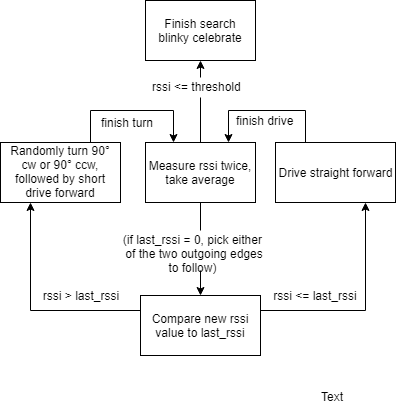
\includegraphics{grad_desc.png}

We also implemented and tested the following improved version that
allows for correction; a car that has just moved forward and detected a
weakened signal does not know whether the beacon to its left or right.
If after turning, the signal is still weaker, it has picked the wrong
turn. This decision process corrects this (same starting state:
\textbf{Measure rssi twice, take average}):

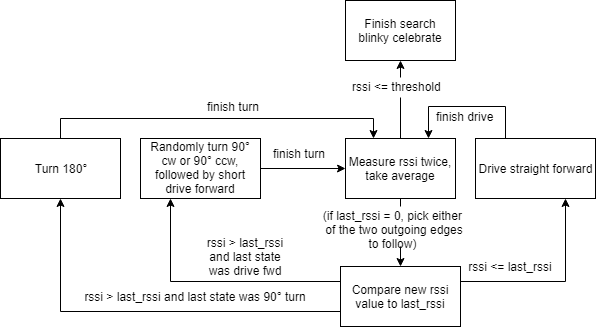
\includegraphics{turn_correction.png}

It did not prove much more accurate than randomized gradient descent,
largely due to noisy readings from IMU and Bluetooth signal strength. As
such, we used the simplified version.

\hypertarget{testing}{%
\subsubsection{Testing}\label{testing}}

\hypertarget{ble-1}{%
\paragraph{BLE}\label{ble-1}}

Once we flashed the Bluetooth chips with the proper firmware, we used
the
\href{https://itunes.apple.com/us/app/lightblue-explorer/id557428110?mt=8}{LightBlue}
app to test communications. Using the app, we could discover the
Bluetooth chips, and send and receive data. By initially using a the
iPhone app, which was known to work, we could debug the Bluetooth chips
in isolation. Once that worked, we had the chips communicate with each
other. Finally, we had the chips take RSSI measurements.

We also experimented with RSSI, as described in
\protect\hyperlink{results}{results}. This data validated the
effectiveness of RSSI as an approximate metric for distance measurement,
though confirmed that it would be highly variable.

\hypertarget{imu-1}{%
\paragraph{IMU}\label{imu-1}}

\begin{itemize}
\tightlist
\item
  Basic I2C: Basic testing was required to ensure I2C communication with
  the chip was working. This included testing the correctness of the I2C
  read and write functions (including the order of starts, restarts, and
  idles in accordance with the I2C protocol and the chip datasheets), as
  well basic parameters like the address of the MPU-9250 and its
  registers.
\item
  Compass I2C: This was more complex, and mostly involved testing the
  usage of the modes of both the MPU-9250 (IMU module) and the AK8963
  (the compass itself). Performance testing was also important here, as
  the compass would not allow rapid reads in quick succession; we
  inserted nops in the
  \texttt{imu\_mag\_read\_data(int\ *\ destination)} for this reason.
\item
  Compass calibration: We tested incrementally, first using hard-coded
  maximum and minimum observed values outputted from the IMU, and then
  with values taken from a self-calibration in which the robot would
  spin in a circle, and the PIC would record the largest and smallest
  values it saw on the X- and Y-axes.
\end{itemize}

\hypertarget{servos-1}{%
\paragraph{Servos}\label{servos-1}}

We tested the functionality of servo code by testing individual
functionality on both the hardware and software side. We tested the
servo code in stages, first implementing control at a fixed speed and
then implementing directional motion and lastly turning. This allowed us
to verify our parts of the code and the functionality of the servos.

\hypertarget{whole-system}{%
\paragraph{Whole system}\label{whole-system}}

\begin{itemize}
\tightlist
\item
  Some subsystem testing was required for the servo with the IMUs, for
  turning/driving straight with feedback. We debugged by reading in IMU
  values via UART and observing the robot's turns.
\item
  We tested extensively with the beacon and two hunters in different
  environments. Most of our initial testing was in a large, open space
  with a few metal tables on the periphery. We later tested in the lab
  in the Digital Lab (Phillips 238), and in the hallway where our demo
  took place. The confined space of the inside of the lab and hallway,
  as well as the presence of more reflective bodies (metal doors,
  tables, people) negatively impacted the performance of our hunters,
  and it was necessary to recalibrate the hunters to work better in the
  demo environment.
\end{itemize}

\hypertarget{results}{%
\subsection{Results}\label{results}}

In most cases, at least 1 of the 2 robots successfully made it to the
base station. However, it was not as reliable as we initially hoped. One
of the main reasons for this was the noise in RSSI measurements.

We expected that RSSI would vary with distance according to the
following relation:

\(\text{RSSI} = A - 10 n \log(d)\)

where \(A\) and \(n\) are RF propagation parameters in dBm, \(d\) is
distance in meters, and RSSI is the measured RSSI in dBm. \footnote{L.
  Peneda, A. Azenha and A. Carvalho, ``Trilateration for indoors
  positioning within the framework of wireless communications,'' 2009
  35th Annual Conference of IEEE Industrial Electronics, Porto, 2009,
  pp.~2732-2737.

  doi: 10.1109/IECON.2009.5415423

  URL:
  \url{http://ieeexplore.ieee.org/stamp/stamp.jsp?tp=\&arnumber=5415423\&isnumber=5414636}}
We experimented with RSSI measurements to determine how well they worked
by taking 2 Bluetooth modules, and measuring the RSSI while changing the
distance between them. One remained stationary on the floor and the
other was moved away from it 1 floor tile (each floor tile is a 1 foot
square) at a time. At each point, we took 3 RSSI measurements and
averaged them. The graph below displays the results:

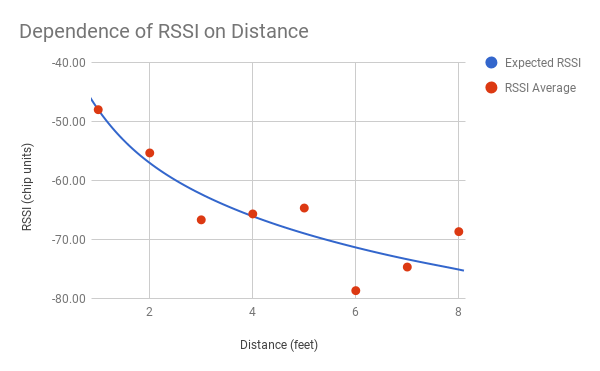
\includegraphics{rssi-chart.png}

While the chip reported RSSI in units proportional to dBm, and we
measured distances in feet, not meters, we could still use the above
formula without worrying about unit conversions. The constants \(A\) and
\(n\), provided we determined them empirically based on the data, would
encode the conversions. As such, we fit the data using the above formula
with \(A=-48\) and \(n=3\), resulting in the blue curve above. While the
general shape of the curve matches, there is significant noise in the
averaged RSSI data. Furthermore, when we tried to reproduce the
measurements, we could not do so precisely -- it seemed to even depend
on where our feet where! See \protect\hyperlink{rssi-data}{Appendix B}
for the source data for the table.

Despite how noisy the RSSI measurements where, the robots were still
able to perform a reasonably accurate gradient descent. In most cases,
at least one of the 2 robots would find the beacon in a matter of
minutes.

\hypertarget{conclusions}{%
\subsection{Conclusions}\label{conclusions}}

This assignment was an interesting exploration into short-range distance
determination using Bluetooth, a generally unconventional approach. We
were warned beforehand about the difficulties in using Bluetooth RSSI, a
measurement particularly susceptible to multipath interference, as a
distance sensor -- both in the papers and reference materials researched
before implementation, as well as by course staff in the early stages of
our project. We worked with the course staff to simplify and stratify
our project into workable milestones. Our final project is a reduced
version of our original plan.

Our hunting bots worked reliably when they stayed within roughly 1 m of
the beacon. After this, they entered the land of shallow gradients: the
signal strength from the beacon (already noisy) would not change very
much, and often only due to noise. The hunting bots normally could never
recover from this. Our bots also worked better in larger, more open
spaces, preferably without metal structures like tables or doors nearby.
Both of these are reasonable given the operating range of BLE 4.0.

We reused some of the code from the
\href{https://people.ece.cornell.edu/land/courses/ece4760/FinalProjects/f2015/dc686_nn233_hz263/final_project_webpage_v2/dc686_nn233_hz263/index.html}{Self-Balancing
Robot} as
\protect\hyperlink{code-and-designs-borrowed-from-others}{cited} in our
references section, and explained in \protect\hyperlink{imu}{IMU}. The
rest of the design is ours, and is not an infringement on intellectual
property. We also used the Bluetooth firmware flashing technique we
discovered on the
\href{http://forum.arduino.cc/index.php?topic=393655.msg2709528\#msg2709528}{Arduino
forums}.

We did not reverse-engineer any technology, and did not encounter any
issues with trademarks or patents. We did not have to sign
non-disclosure to get a sample part. We hope to further polish our
findings and report, and will aim to publish them in a print magazine,
ideally as a part of ECE 4920.

There are many potential avenues for improvements or further
development. In addition to more circumstantial difficulties encountered
during the project work period (such as extremely unbalanced servos,
where one always ran faster than the other), two areas of potential
improvement are as follows:

\begin{itemize}
\tightlist
\item
  \emph{Communication between the two robots}. While Bluetooth may not
  offer good distance measurement via RSSI, it can be used for reliable
  communication between modules. It would be straightforward for one
  hunting robot to inform the other whether it believes it is
  approaching the beacon or not. In the simplest case, a hunting robot
  that is approaching, or already at, the beacon can provide a second
  point of reference for a currently hunting robot.
\item
  \emph{More complete usage of IMU}. A lot of development time was spent
  simply on getting the PIC to compass communication running, and not
  much time was spent on calibrating the sensor or processing the data.
  In further stages of this project, we could continue to work towards
  dead reckoning of the mobile robots. This, paired with inter-swarm
  communication, would make for a much more sophisticated and likely
  much more efficient system. (Of course, this does not resolve the
  shallow gradients problem -- but it would allow the approach to the
  beacon to be much faster.)
\end{itemize}

\hypertarget{appendices}{%
\subsection{Appendices}\label{appendices}}

\hypertarget{appendix-c-schematics}{%
\subsubsection{Appendix A: Data}\label{appendix-c-schematics}}

\hypertarget{rssi-data}{%
\paragraph{RSSI data}\label{rssi-data}}

\begin{longtable}[]{@{}llllll@{}}
\toprule
Distance (feet) & RSSI A & RSSI B & RSSI C & RSSI Average & Expected
RSSI\tabularnewline
\midrule
\endhead
1 & -48 & -48 & -48 & -48.00 & -48.00\tabularnewline
2 & -56 & -58 & -52 & -55.33 & -57.03\tabularnewline
3 & -66 & -66 & -68 & -66.67 & -62.31\tabularnewline
4 & -64 & -68 & -65 & -65.67 & -66.06\tabularnewline
5 & -60 & -70 & -64 & -64.67 & -68.97\tabularnewline
6 & -80 & -80 & -76 & -78.67 & -71.34\tabularnewline
7 & -80 & -79 & -65 & -74.67 & -73.35\tabularnewline
8 & -68 & -66 & -72 & -68.67 & -75.09\tabularnewline
\bottomrule
\end{longtable}

\hypertarget{appendix-c-schematics}{%
\subsubsection{Appendix B: Schematics}\label{appendix-c-schematics}}

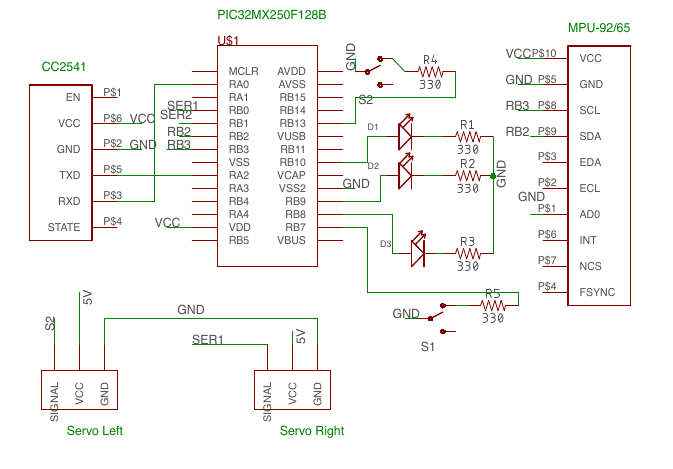
\includegraphics{schematic.png}

\hypertarget{appendix-d-bill-of-materials}{%
\subsubsection{Appendix D: Bill Of
Materials}\label{appendix-d-bill-of-materials}}

\begin{longtable}[]{@{}lllllll@{}}
\toprule
\begin{minipage}[b]{0.15\columnwidth}\raggedright
Name\strut
\end{minipage} & \begin{minipage}[b]{0.15\columnwidth}\raggedright
Manufacturer Part Number\strut
\end{minipage} & \begin{minipage}[b]{0.10\columnwidth}\raggedright
Vendor\strut
\end{minipage} & \begin{minipage}[b]{0.17\columnwidth}\raggedright
Vendor Part Number\strut
\end{minipage} & \begin{minipage}[b]{0.11\columnwidth}\raggedright
Quantity\strut
\end{minipage} & \begin{minipage}[b]{0.06\columnwidth}\raggedright
Unit Cost\strut
\end{minipage} & \begin{minipage}[b]{0.07\columnwidth}\raggedright
Total Cost\strut
\end{minipage}\tabularnewline
\midrule
\endhead
\begin{minipage}[t]{0.15\columnwidth}\raggedright
BLE 4.0 Module (TI CC2541)\strut
\end{minipage} & \begin{minipage}[t]{0.15\columnwidth}\raggedright
HM-10\strut
\end{minipage} & \begin{minipage}[t]{0.10\columnwidth}\raggedright
\href{https://www.ebay.com/itm/AT-09-BLE-Bluetooth-4-0-Uart-Transceiver-Module-CC2541-Central-Switching-HM-10/142425748901?ssPageName=STRK\%3AMEBIDX\%3AIT\&_trksid=p2057872.m2749.l2649}{Ebay}\strut
\end{minipage} & \begin{minipage}[t]{0.17\columnwidth}\raggedright
142425748901\strut
\end{minipage} & \begin{minipage}[t]{0.11\columnwidth}\raggedright
3\strut
\end{minipage} & \begin{minipage}[t]{0.06\columnwidth}\raggedright
\$3.99\strut
\end{minipage} & \begin{minipage}[t]{0.07\columnwidth}\raggedright
\$11.97\strut
\end{minipage}\tabularnewline
\begin{minipage}[t]{0.15\columnwidth}\raggedright
FEETECH FS90R (pack of 2) Continuous Rotation Robotic Servo\strut
\end{minipage} & \begin{minipage}[t]{0.15\columnwidth}\raggedright
FS90R\strut
\end{minipage} & \begin{minipage}[t]{0.10\columnwidth}\raggedright
\href{https://www.amazon.com/gp/product/B074BFQC3Q/ref=oh_aui_detailpage_o06_s00?ie=UTF8\&psc=1}{Amazon}\strut
\end{minipage} & \begin{minipage}[t]{0.17\columnwidth}\raggedright
B074BFQC3Q\strut
\end{minipage} & \begin{minipage}[t]{0.11\columnwidth}\raggedright
2\strut
\end{minipage} & \begin{minipage}[t]{0.06\columnwidth}\raggedright
\$12.39\strut
\end{minipage} & \begin{minipage}[t]{0.07\columnwidth}\raggedright
\$24.78\strut
\end{minipage}\tabularnewline
\begin{minipage}[t]{0.15\columnwidth}\raggedright
HiLetgo 9-Axis 9 DOF 16 Bit Gyroscope Acceleration Magnetic Sensor\strut
\end{minipage} & \begin{minipage}[t]{0.15\columnwidth}\raggedright
MPU-9250\strut
\end{minipage} & \begin{minipage}[t]{0.10\columnwidth}\raggedright
\href{https://www.amazon.com/HiLetgo-Gyroscope-Acceleration-Accelerator-Magnetometer/dp/B01I1J0Z7Y/ref=redir_mobile_desktop?_encoding=UTF8\&dpID=51nl2fcMh6L\&dpPl=1\&keywords=mpu\%209250\&pi=AC_SX236_SY340_QL65\&qid=1512564044\&ref=plSrch\&ref_=mp_s_a_1_3\&sr=8-3}{Amazon}\strut
\end{minipage} & \begin{minipage}[t]{0.17\columnwidth}\raggedright
B01I1J0Z7Y\strut
\end{minipage} & \begin{minipage}[t]{0.11\columnwidth}\raggedright
2\strut
\end{minipage} & \begin{minipage}[t]{0.06\columnwidth}\raggedright
\$8.49\strut
\end{minipage} & \begin{minipage}[t]{0.07\columnwidth}\raggedright
\$16.98\strut
\end{minipage}\tabularnewline
\begin{minipage}[t]{0.15\columnwidth}\raggedright
Small board\strut
\end{minipage} & \begin{minipage}[t]{0.15\columnwidth}\raggedright
--\strut
\end{minipage} & \begin{minipage}[t]{0.10\columnwidth}\raggedright
Lab rental\strut
\end{minipage} & \begin{minipage}[t]{0.17\columnwidth}\raggedright
--\strut
\end{minipage} & \begin{minipage}[t]{0.11\columnwidth}\raggedright
3\strut
\end{minipage} & \begin{minipage}[t]{0.06\columnwidth}\raggedright
\$5.00\strut
\end{minipage} & \begin{minipage}[t]{0.07\columnwidth}\raggedright
\$15.00\strut
\end{minipage}\tabularnewline
\begin{minipage}[t]{0.15\columnwidth}\raggedright
PIC32MX250F128B\strut
\end{minipage} & \begin{minipage}[t]{0.15\columnwidth}\raggedright
PIC32MX250F128B\strut
\end{minipage} & \begin{minipage}[t]{0.10\columnwidth}\raggedright
Lab rental\strut
\end{minipage} & \begin{minipage}[t]{0.17\columnwidth}\raggedright
--\strut
\end{minipage} & \begin{minipage}[t]{0.11\columnwidth}\raggedright
3\strut
\end{minipage} & \begin{minipage}[t]{0.06\columnwidth}\raggedright
\$5.00\strut
\end{minipage} & \begin{minipage}[t]{0.07\columnwidth}\raggedright
\$15.00\strut
\end{minipage}\tabularnewline
\begin{minipage}[t]{0.15\columnwidth}\raggedright
6-inch Protoboard\strut
\end{minipage} & \begin{minipage}[t]{0.15\columnwidth}\raggedright
--\strut
\end{minipage} & \begin{minipage}[t]{0.10\columnwidth}\raggedright
Lab rental\strut
\end{minipage} & \begin{minipage}[t]{0.17\columnwidth}\raggedright
--\strut
\end{minipage} & \begin{minipage}[t]{0.11\columnwidth}\raggedright
3\strut
\end{minipage} & \begin{minipage}[t]{0.06\columnwidth}\raggedright
\$2.50\strut
\end{minipage} & \begin{minipage}[t]{0.07\columnwidth}\raggedright
\$7.50\strut
\end{minipage}\tabularnewline
\begin{minipage}[t]{0.15\columnwidth}\raggedright
Male header pins\strut
\end{minipage} & \begin{minipage}[t]{0.15\columnwidth}\raggedright
--\strut
\end{minipage} & \begin{minipage}[t]{0.10\columnwidth}\raggedright
Lab\strut
\end{minipage} & \begin{minipage}[t]{0.17\columnwidth}\raggedright
--\strut
\end{minipage} & \begin{minipage}[t]{0.11\columnwidth}\raggedright
129\strut
\end{minipage} & \begin{minipage}[t]{0.06\columnwidth}\raggedright
\$0.05\strut
\end{minipage} & \begin{minipage}[t]{0.07\columnwidth}\raggedright
\$6.45\strut
\end{minipage}\tabularnewline
\bottomrule
\end{longtable}

\textbf{Total:} \$97.68

\hypertarget{references}{%
\subsubsection{References}\label{references}}

\hypertarget{data-sheets}{%
\paragraph{Data sheets}\label{data-sheets}}

\begin{itemize}
\tightlist
\item
  \href{https://www.invensense.com/wp-content/uploads/2015/02/PS-MPU-9250A-01-v1.1.pdf}{MPU-9250}
  and
  \href{https://cdn.sparkfun.com/assets/learn_tutorials/5/5/0/MPU-9250-Register-Map.pdf}{its
  register map}.
\item
  \href{https://www.akm.com/akm/en/file/datasheet/AK8963C.pdf}{3-axis
  Electronic Compass on IMU}.
\item
  \href{http://www.jnhuamao.cn/bluetooth40_en.zip}{HM-10 (Bluetooth
  breakout module \& firmware)}. The ZIP contains the original data
  sheet, as well as other documentation.
  \href{http://fab.cba.mit.edu/classes/863.15/doc/tutorials/programming/bluetooth/bluetooth40_en.pdf}{MIT
  has a PDF} available, which may me out of date, but is easier to get
  to.
\item
  \href{http://ww1.microchip.com/downloads/en/DeviceDoc/60001168J.pdf}{PIC32MX250}.
\end{itemize}

\hypertarget{code-and-designs-borrowed-from-others}{%
\paragraph{Code and designs borrowed from
others}\label{code-and-designs-borrowed-from-others}}

\begin{itemize}
\tightlist
\item
  \href{https://people.ece.cornell.edu/land/courses/ece4760/FinalProjects/f2015/dc686_nn233_hz263/final_project_webpage_v2/dc686_nn233_hz263/index.html}{Self-Balancing
  Robot} by Desmond Caulley (dc686@cornell.edu), Nadav Nehoran
  (nn233@cornell.edu), Sherry Zhao (hz263@cornell.edu). In particular,
  we borrowed extensively from their
  \href{https://people.ece.cornell.edu/land/courses/ece4760/FinalProjects/f2015/dc686_nn233_hz263/final_project_webpage_v2/dc686_nn233_hz263/dc686_nn233_hz263/i2c_helper.h}{i2c\_helper.h}.
\end{itemize}

\hypertarget{other}{%
\paragraph{Other}\label{other}}

\begin{itemize}
\tightlist
\item
  \href{http://people.ece.cornell.edu/land/courses/ece4760/}{ECE 4760
  Website} by Bruce Land
\item
  Website template:
  \url{https://github.com/tajmone/pandoc-goodies/tree/master/templates/html5/github}.
\end{itemize}

\end{document}
